% Options for packages loaded elsewhere
\PassOptionsToPackage{unicode}{hyperref}
\PassOptionsToPackage{hyphens}{url}
\PassOptionsToPackage{dvipsnames,svgnames,x11names}{xcolor}
%
\documentclass[
  letterpaper,
  DIV=11,
  numbers=noendperiod]{scrartcl}

\usepackage{amsmath,amssymb}
\usepackage{iftex}
\ifPDFTeX
  \usepackage[T1]{fontenc}
  \usepackage[utf8]{inputenc}
  \usepackage{textcomp} % provide euro and other symbols
\else % if luatex or xetex
  \usepackage{unicode-math}
  \defaultfontfeatures{Scale=MatchLowercase}
  \defaultfontfeatures[\rmfamily]{Ligatures=TeX,Scale=1}
\fi
\usepackage{lmodern}
\ifPDFTeX\else  
    % xetex/luatex font selection
\fi
% Use upquote if available, for straight quotes in verbatim environments
\IfFileExists{upquote.sty}{\usepackage{upquote}}{}
\IfFileExists{microtype.sty}{% use microtype if available
  \usepackage[]{microtype}
  \UseMicrotypeSet[protrusion]{basicmath} % disable protrusion for tt fonts
}{}
\makeatletter
\@ifundefined{KOMAClassName}{% if non-KOMA class
  \IfFileExists{parskip.sty}{%
    \usepackage{parskip}
  }{% else
    \setlength{\parindent}{0pt}
    \setlength{\parskip}{6pt plus 2pt minus 1pt}}
}{% if KOMA class
  \KOMAoptions{parskip=half}}
\makeatother
\usepackage{xcolor}
\setlength{\emergencystretch}{3em} % prevent overfull lines
\setcounter{secnumdepth}{-\maxdimen} % remove section numbering
% Make \paragraph and \subparagraph free-standing
\makeatletter
\ifx\paragraph\undefined\else
  \let\oldparagraph\paragraph
  \renewcommand{\paragraph}{
    \@ifstar
      \xxxParagraphStar
      \xxxParagraphNoStar
  }
  \newcommand{\xxxParagraphStar}[1]{\oldparagraph*{#1}\mbox{}}
  \newcommand{\xxxParagraphNoStar}[1]{\oldparagraph{#1}\mbox{}}
\fi
\ifx\subparagraph\undefined\else
  \let\oldsubparagraph\subparagraph
  \renewcommand{\subparagraph}{
    \@ifstar
      \xxxSubParagraphStar
      \xxxSubParagraphNoStar
  }
  \newcommand{\xxxSubParagraphStar}[1]{\oldsubparagraph*{#1}\mbox{}}
  \newcommand{\xxxSubParagraphNoStar}[1]{\oldsubparagraph{#1}\mbox{}}
\fi
\makeatother

\usepackage{color}
\usepackage{fancyvrb}
\newcommand{\VerbBar}{|}
\newcommand{\VERB}{\Verb[commandchars=\\\{\}]}
\DefineVerbatimEnvironment{Highlighting}{Verbatim}{commandchars=\\\{\}}
% Add ',fontsize=\small' for more characters per line
\usepackage{framed}
\definecolor{shadecolor}{RGB}{241,243,245}
\newenvironment{Shaded}{\begin{snugshade}}{\end{snugshade}}
\newcommand{\AlertTok}[1]{\textcolor[rgb]{0.68,0.00,0.00}{#1}}
\newcommand{\AnnotationTok}[1]{\textcolor[rgb]{0.37,0.37,0.37}{#1}}
\newcommand{\AttributeTok}[1]{\textcolor[rgb]{0.40,0.45,0.13}{#1}}
\newcommand{\BaseNTok}[1]{\textcolor[rgb]{0.68,0.00,0.00}{#1}}
\newcommand{\BuiltInTok}[1]{\textcolor[rgb]{0.00,0.23,0.31}{#1}}
\newcommand{\CharTok}[1]{\textcolor[rgb]{0.13,0.47,0.30}{#1}}
\newcommand{\CommentTok}[1]{\textcolor[rgb]{0.37,0.37,0.37}{#1}}
\newcommand{\CommentVarTok}[1]{\textcolor[rgb]{0.37,0.37,0.37}{\textit{#1}}}
\newcommand{\ConstantTok}[1]{\textcolor[rgb]{0.56,0.35,0.01}{#1}}
\newcommand{\ControlFlowTok}[1]{\textcolor[rgb]{0.00,0.23,0.31}{\textbf{#1}}}
\newcommand{\DataTypeTok}[1]{\textcolor[rgb]{0.68,0.00,0.00}{#1}}
\newcommand{\DecValTok}[1]{\textcolor[rgb]{0.68,0.00,0.00}{#1}}
\newcommand{\DocumentationTok}[1]{\textcolor[rgb]{0.37,0.37,0.37}{\textit{#1}}}
\newcommand{\ErrorTok}[1]{\textcolor[rgb]{0.68,0.00,0.00}{#1}}
\newcommand{\ExtensionTok}[1]{\textcolor[rgb]{0.00,0.23,0.31}{#1}}
\newcommand{\FloatTok}[1]{\textcolor[rgb]{0.68,0.00,0.00}{#1}}
\newcommand{\FunctionTok}[1]{\textcolor[rgb]{0.28,0.35,0.67}{#1}}
\newcommand{\ImportTok}[1]{\textcolor[rgb]{0.00,0.46,0.62}{#1}}
\newcommand{\InformationTok}[1]{\textcolor[rgb]{0.37,0.37,0.37}{#1}}
\newcommand{\KeywordTok}[1]{\textcolor[rgb]{0.00,0.23,0.31}{\textbf{#1}}}
\newcommand{\NormalTok}[1]{\textcolor[rgb]{0.00,0.23,0.31}{#1}}
\newcommand{\OperatorTok}[1]{\textcolor[rgb]{0.37,0.37,0.37}{#1}}
\newcommand{\OtherTok}[1]{\textcolor[rgb]{0.00,0.23,0.31}{#1}}
\newcommand{\PreprocessorTok}[1]{\textcolor[rgb]{0.68,0.00,0.00}{#1}}
\newcommand{\RegionMarkerTok}[1]{\textcolor[rgb]{0.00,0.23,0.31}{#1}}
\newcommand{\SpecialCharTok}[1]{\textcolor[rgb]{0.37,0.37,0.37}{#1}}
\newcommand{\SpecialStringTok}[1]{\textcolor[rgb]{0.13,0.47,0.30}{#1}}
\newcommand{\StringTok}[1]{\textcolor[rgb]{0.13,0.47,0.30}{#1}}
\newcommand{\VariableTok}[1]{\textcolor[rgb]{0.07,0.07,0.07}{#1}}
\newcommand{\VerbatimStringTok}[1]{\textcolor[rgb]{0.13,0.47,0.30}{#1}}
\newcommand{\WarningTok}[1]{\textcolor[rgb]{0.37,0.37,0.37}{\textit{#1}}}

\providecommand{\tightlist}{%
  \setlength{\itemsep}{0pt}\setlength{\parskip}{0pt}}\usepackage{longtable,booktabs,array}
\usepackage{calc} % for calculating minipage widths
% Correct order of tables after \paragraph or \subparagraph
\usepackage{etoolbox}
\makeatletter
\patchcmd\longtable{\par}{\if@noskipsec\mbox{}\fi\par}{}{}
\makeatother
% Allow footnotes in longtable head/foot
\IfFileExists{footnotehyper.sty}{\usepackage{footnotehyper}}{\usepackage{footnote}}
\makesavenoteenv{longtable}
\usepackage{graphicx}
\makeatletter
\def\maxwidth{\ifdim\Gin@nat@width>\linewidth\linewidth\else\Gin@nat@width\fi}
\def\maxheight{\ifdim\Gin@nat@height>\textheight\textheight\else\Gin@nat@height\fi}
\makeatother
% Scale images if necessary, so that they will not overflow the page
% margins by default, and it is still possible to overwrite the defaults
% using explicit options in \includegraphics[width, height, ...]{}
\setkeys{Gin}{width=\maxwidth,height=\maxheight,keepaspectratio}
% Set default figure placement to htbp
\makeatletter
\def\fps@figure{htbp}
\makeatother

\KOMAoption{captions}{tableheading}
\makeatletter
\@ifpackageloaded{caption}{}{\usepackage{caption}}
\AtBeginDocument{%
\ifdefined\contentsname
  \renewcommand*\contentsname{Table of contents}
\else
  \newcommand\contentsname{Table of contents}
\fi
\ifdefined\listfigurename
  \renewcommand*\listfigurename{List of Figures}
\else
  \newcommand\listfigurename{List of Figures}
\fi
\ifdefined\listtablename
  \renewcommand*\listtablename{List of Tables}
\else
  \newcommand\listtablename{List of Tables}
\fi
\ifdefined\figurename
  \renewcommand*\figurename{Figure}
\else
  \newcommand\figurename{Figure}
\fi
\ifdefined\tablename
  \renewcommand*\tablename{Table}
\else
  \newcommand\tablename{Table}
\fi
}
\@ifpackageloaded{float}{}{\usepackage{float}}
\floatstyle{ruled}
\@ifundefined{c@chapter}{\newfloat{codelisting}{h}{lop}}{\newfloat{codelisting}{h}{lop}[chapter]}
\floatname{codelisting}{Listing}
\newcommand*\listoflistings{\listof{codelisting}{List of Listings}}
\makeatother
\makeatletter
\makeatother
\makeatletter
\@ifpackageloaded{caption}{}{\usepackage{caption}}
\@ifpackageloaded{subcaption}{}{\usepackage{subcaption}}
\makeatother

\ifLuaTeX
  \usepackage{selnolig}  % disable illegal ligatures
\fi
\usepackage{bookmark}

\IfFileExists{xurl.sty}{\usepackage{xurl}}{} % add URL line breaks if available
\urlstyle{same} % disable monospaced font for URLs
\hypersetup{
  pdftitle={EDA Analysis on final dataset},
  colorlinks=true,
  linkcolor={blue},
  filecolor={Maroon},
  citecolor={Blue},
  urlcolor={Blue},
  pdfcreator={LaTeX via pandoc}}


\title{EDA Analysis on final dataset}
\author{}
\date{}

\begin{document}
\maketitle


\subsection{Quarto}\label{quarto}

\subsection{Data Loading and Initial
Overview}\label{data-loading-and-initial-overview}

\begin{Shaded}
\begin{Highlighting}[]
\CommentTok{\# Load necessary libraries}
\FunctionTok{library}\NormalTok{(tidyverse)}
\end{Highlighting}
\end{Shaded}

\begin{verbatim}
-- Attaching core tidyverse packages ------------------------ tidyverse 2.0.0 --
v dplyr     1.1.4     v readr     2.1.5
v forcats   1.0.0     v stringr   1.5.0
v ggplot2   3.4.3     v tibble    3.2.1
v lubridate 1.9.3     v tidyr     1.3.1
v purrr     1.0.2     
-- Conflicts ------------------------------------------ tidyverse_conflicts() --
x dplyr::filter() masks stats::filter()
x dplyr::lag()    masks stats::lag()
i Use the conflicted package (<http://conflicted.r-lib.org/>) to force all conflicts to become errors
\end{verbatim}

\begin{Shaded}
\begin{Highlighting}[]
\FunctionTok{library}\NormalTok{(naniar)}
\FunctionTok{library}\NormalTok{(corrplot)}
\end{Highlighting}
\end{Shaded}

\begin{verbatim}
Warning: package 'corrplot' was built under R version 4.3.3
\end{verbatim}

\begin{verbatim}
corrplot 0.94 loaded
\end{verbatim}

\begin{Shaded}
\begin{Highlighting}[]
\FunctionTok{library}\NormalTok{(ggplot2)}
\FunctionTok{library}\NormalTok{(dplyr)}

\CommentTok{\# Load the dataset}
\NormalTok{data }\OtherTok{\textless{}{-}} \FunctionTok{read.csv}\NormalTok{(}\StringTok{"/Users/wangsiwei/Desktop/version\_control/armed\_conflict/data/analytical/finaldata.csv"}\NormalTok{, }\AttributeTok{header =} \ConstantTok{TRUE}\NormalTok{)}

\CommentTok{\# Display the first few rows}
\FunctionTok{head}\NormalTok{(data)}
\end{Highlighting}
\end{Shaded}

\begin{verbatim}
  country_name ISO        region year   gdp1000 OECD OECD2023  popdens    urban
1  Afghanistan AFG Southern Asia 2000        NA    0        0 14.13654 16.25324
2  Afghanistan AFG Southern Asia 2001        NA    0        0 14.23156 16.25661
3  Afghanistan AFG Southern Asia 2002 0.1835328    0        0 14.32270 16.42654
4  Afghanistan AFG Southern Asia 2003 0.2004626    0        0 14.40691 16.60701
5  Afghanistan AFG Southern Asia 2004 0.2216576    0        0 15.21947 16.71367
6  Afghanistan AFG Southern Asia 2005 0.2550551    0        0 15.33619 16.85096
    agedep male_edu     temp rainfall1000 totdeath armconf1 matmor infmor
1 108.3466 2.762086 12.69959    0.2763704     5065        1   1450   90.5
2 108.9899 2.856936 12.85570    0.2793079     5394        1   1390   87.9
3 109.3472 2.954241 12.71081    0.3805710     5553        1   1300   85.3
4 109.4475 3.054121 12.16592    0.4288939     1157        1   1240   82.7
5 109.2868 3.156706 13.04643    0.3754336      944        1   1180   80.0
6 107.9646 3.262133 12.23141    0.4415680      817        1   1140   77.3
  neomor un5mor drought earthquake
1   60.9  129.2       1          0
2   59.7  125.2       0          1
3   58.5  121.1       0          1
4   57.2  116.9       0          1
5   55.9  112.6       0          1
6   54.6  108.4       0          1
\end{verbatim}

\begin{Shaded}
\begin{Highlighting}[]
\CommentTok{\# Overview of the structure of the dataset}
\FunctionTok{str}\NormalTok{(data)}
\end{Highlighting}
\end{Shaded}

\begin{verbatim}
'data.frame':   3720 obs. of  21 variables:
 $ country_name: chr  "Afghanistan" "Afghanistan" "Afghanistan" "Afghanistan" ...
 $ ISO         : chr  "AFG" "AFG" "AFG" "AFG" ...
 $ region      : chr  "Southern Asia" "Southern Asia" "Southern Asia" "Southern Asia" ...
 $ year        : int  2000 2001 2002 2003 2004 2005 2006 2007 2008 2009 ...
 $ gdp1000     : num  NA NA 0.184 0.2 0.222 ...
 $ OECD        : int  0 0 0 0 0 0 0 0 0 0 ...
 $ OECD2023    : int  0 0 0 0 0 0 0 0 0 0 ...
 $ popdens     : num  14.1 14.2 14.3 14.4 15.2 ...
 $ urban       : num  16.3 16.3 16.4 16.6 16.7 ...
 $ agedep      : num  108 109 109 109 109 ...
 $ male_edu    : num  2.76 2.86 2.95 3.05 3.16 ...
 $ temp        : num  12.7 12.9 12.7 12.2 13 ...
 $ rainfall1000: num  0.276 0.279 0.381 0.429 0.375 ...
 $ totdeath    : int  5065 5394 5553 1157 944 817 1711 4982 7020 5660 ...
 $ armconf1    : int  1 1 1 1 1 1 1 1 1 1 ...
 $ matmor      : int  1450 1390 1300 1240 1180 1140 1120 1090 1030 993 ...
 $ infmor      : num  90.5 87.9 85.3 82.7 80 77.3 74.6 71.9 69.2 66.7 ...
 $ neomor      : num  60.9 59.7 58.5 57.2 55.9 54.6 53.2 51.7 50.3 48.9 ...
 $ un5mor      : num  129 125 121 117 113 ...
 $ drought     : int  1 0 0 0 0 0 1 0 1 0 ...
 $ earthquake  : int  0 1 1 1 1 1 1 0 0 1 ...
\end{verbatim}

\begin{Shaded}
\begin{Highlighting}[]
\CommentTok{\# Summary statistics}
\FunctionTok{summary}\NormalTok{(data)}
\end{Highlighting}
\end{Shaded}

\begin{verbatim}
 country_name           ISO               region               year     
 Length:3720        Length:3720        Length:3720        Min.   :2000  
 Class :character   Class :character   Class :character   1st Qu.:2005  
 Mode  :character   Mode  :character   Mode  :character   Median :2010  
                                                          Mean   :2010  
                                                          3rd Qu.:2014  
                                                          Max.   :2019  
                                                                        
    gdp1000              OECD          OECD2023         popdens     
 Min.   :  0.1105   Min.   :0.000   Min.   :0.0000   Min.   : 0.00  
 1st Qu.:  1.2383   1st Qu.:0.000   1st Qu.:0.0000   1st Qu.:14.79  
 Median :  4.0719   Median :0.000   Median :0.0000   Median :27.52  
 Mean   : 11.4917   Mean   :0.171   Mean   :0.1882   Mean   :30.57  
 3rd Qu.: 13.1531   3rd Qu.:0.000   3rd Qu.:0.0000   3rd Qu.:40.72  
 Max.   :123.6787   Max.   :1.000   Max.   :1.0000   Max.   :99.86  
 NA's   :62                                          NA's   :20     
     urban             agedep          male_edu           temp       
 Min.   : 0.1025   Min.   : 16.17   Min.   : 1.067   Min.   :-2.405  
 1st Qu.:17.2872   1st Qu.: 47.94   1st Qu.: 5.904   1st Qu.:12.928  
 Median :30.2535   Median : 55.51   Median : 8.368   Median :21.958  
 Mean   :30.6948   Mean   : 61.94   Mean   : 8.258   Mean   :19.625  
 3rd Qu.:41.6558   3rd Qu.: 77.11   3rd Qu.:10.849   3rd Qu.:25.869  
 Max.   :93.4135   Max.   :111.48   Max.   :14.441   Max.   :29.676  
 NA's   :20                         NA's   :20       NA's   :20      
  rainfall1000        totdeath          armconf1          matmor      
 Min.   :0.01993   Min.   :    0.0   Min.   :0.0000   Min.   :   2.0  
 1st Qu.:0.59146   1st Qu.:    0.0   1st Qu.:0.0000   1st Qu.:  17.0  
 Median :1.01288   Median :    0.0   Median :0.0000   Median :  66.0  
 Mean   :1.20216   Mean   :  361.1   Mean   :0.1892   Mean   : 210.6  
 3rd Qu.:1.68706   3rd Qu.:    2.0   3rd Qu.:0.0000   3rd Qu.: 299.8  
 Max.   :4.71081   Max.   :78644.0   Max.   :1.0000   Max.   :2480.0  
 NA's   :20                                           NA's   :426     
     infmor           neomor          un5mor          drought       
 Min.   :  1.60   Min.   : 0.80   Min.   :  2.00   Min.   :0.00000  
 1st Qu.:  7.60   1st Qu.: 4.90   1st Qu.:  9.00   1st Qu.:0.00000  
 Median : 18.90   Median :12.10   Median : 22.20   Median :0.00000  
 Mean   : 28.90   Mean   :16.18   Mean   : 40.50   Mean   :0.08737  
 3rd Qu.: 44.52   3rd Qu.:25.32   3rd Qu.: 61.33   3rd Qu.:0.00000  
 Max.   :138.10   Max.   :60.90   Max.   :224.90   Max.   :1.00000  
 NA's   :20       NA's   :20      NA's   :20                        
   earthquake     
 Min.   :0.00000  
 1st Qu.:0.00000  
 Median :0.00000  
 Mean   :0.08333  
 3rd Qu.:0.00000  
 Max.   :1.00000  
                  
\end{verbatim}

\textbf{Insight}: - The dataset contains various economic, demographic,
and environmental indicators. - The structure overview shows numeric
variables like \texttt{gdp1000}, \texttt{popdens}, and mortality rates.
- The summary statistics reveal missing values in some columns (like
GDP), which may need further attention.

\begin{Shaded}
\begin{Highlighting}[]
\CommentTok{\# Check for missing values}
\NormalTok{missing\_values }\OtherTok{\textless{}{-}} \FunctionTok{colSums}\NormalTok{(}\FunctionTok{is.na}\NormalTok{(data))}
\NormalTok{missing\_values}
\end{Highlighting}
\end{Shaded}

\begin{verbatim}
country_name          ISO       region         year      gdp1000         OECD 
           0            0            0            0           62            0 
    OECD2023      popdens        urban       agedep     male_edu         temp 
           0           20           20            0           20           20 
rainfall1000     totdeath     armconf1       matmor       infmor       neomor 
          20            0            0          426           20           20 
      un5mor      drought   earthquake 
          20            0            0 
\end{verbatim}

\textbf{Insight}: - We can observe missing values in several columns,
especially \texttt{gdp1000}. Handling these missing values will be
essential for analysis and interpretation.

\begin{Shaded}
\begin{Highlighting}[]
\CommentTok{\# Descriptive statistics for numeric variables}
\NormalTok{numeric\_vars }\OtherTok{\textless{}{-}}\NormalTok{ data }\SpecialCharTok{\%\textgreater{}\%} \FunctionTok{select}\NormalTok{(}\FunctionTok{where}\NormalTok{(is.numeric))}
\FunctionTok{summary}\NormalTok{(numeric\_vars)}
\end{Highlighting}
\end{Shaded}

\begin{verbatim}
      year         gdp1000              OECD          OECD2023     
 Min.   :2000   Min.   :  0.1105   Min.   :0.000   Min.   :0.0000  
 1st Qu.:2005   1st Qu.:  1.2383   1st Qu.:0.000   1st Qu.:0.0000  
 Median :2010   Median :  4.0719   Median :0.000   Median :0.0000  
 Mean   :2010   Mean   : 11.4917   Mean   :0.171   Mean   :0.1882  
 3rd Qu.:2014   3rd Qu.: 13.1531   3rd Qu.:0.000   3rd Qu.:0.0000  
 Max.   :2019   Max.   :123.6787   Max.   :1.000   Max.   :1.0000  
                NA's   :62                                         
    popdens          urban             agedep          male_edu     
 Min.   : 0.00   Min.   : 0.1025   Min.   : 16.17   Min.   : 1.067  
 1st Qu.:14.79   1st Qu.:17.2872   1st Qu.: 47.94   1st Qu.: 5.904  
 Median :27.52   Median :30.2535   Median : 55.51   Median : 8.368  
 Mean   :30.57   Mean   :30.6948   Mean   : 61.94   Mean   : 8.258  
 3rd Qu.:40.72   3rd Qu.:41.6558   3rd Qu.: 77.11   3rd Qu.:10.849  
 Max.   :99.86   Max.   :93.4135   Max.   :111.48   Max.   :14.441  
 NA's   :20      NA's   :20                         NA's   :20      
      temp         rainfall1000        totdeath          armconf1     
 Min.   :-2.405   Min.   :0.01993   Min.   :    0.0   Min.   :0.0000  
 1st Qu.:12.928   1st Qu.:0.59146   1st Qu.:    0.0   1st Qu.:0.0000  
 Median :21.958   Median :1.01288   Median :    0.0   Median :0.0000  
 Mean   :19.625   Mean   :1.20216   Mean   :  361.1   Mean   :0.1892  
 3rd Qu.:25.869   3rd Qu.:1.68706   3rd Qu.:    2.0   3rd Qu.:0.0000  
 Max.   :29.676   Max.   :4.71081   Max.   :78644.0   Max.   :1.0000  
 NA's   :20       NA's   :20                                          
     matmor           infmor           neomor          un5mor      
 Min.   :   2.0   Min.   :  1.60   Min.   : 0.80   Min.   :  2.00  
 1st Qu.:  17.0   1st Qu.:  7.60   1st Qu.: 4.90   1st Qu.:  9.00  
 Median :  66.0   Median : 18.90   Median :12.10   Median : 22.20  
 Mean   : 210.6   Mean   : 28.90   Mean   :16.18   Mean   : 40.50  
 3rd Qu.: 299.8   3rd Qu.: 44.52   3rd Qu.:25.32   3rd Qu.: 61.33  
 Max.   :2480.0   Max.   :138.10   Max.   :60.90   Max.   :224.90  
 NA's   :426      NA's   :20       NA's   :20      NA's   :20      
    drought          earthquake     
 Min.   :0.00000   Min.   :0.00000  
 1st Qu.:0.00000   1st Qu.:0.00000  
 Median :0.00000   Median :0.00000  
 Mean   :0.08737   Mean   :0.08333  
 3rd Qu.:0.00000   3rd Qu.:0.00000  
 Max.   :1.00000   Max.   :1.00000  
                                    
\end{verbatim}

\textbf{Insight}: - The summary confirms wide variability across numeric
variables. For example, \texttt{gdp1000} shows a high range of values,
likely due to differences in economic output among countries.

\subsection{Univariate Analysis}\label{univariate-analysis}

\begin{Shaded}
\begin{Highlighting}[]
\CommentTok{\# GDP distribution}
\FunctionTok{ggplot}\NormalTok{(data, }\FunctionTok{aes}\NormalTok{(}\AttributeTok{x =}\NormalTok{ gdp1000)) }\SpecialCharTok{+} 
  \FunctionTok{geom\_histogram}\NormalTok{(}\AttributeTok{binwidth =} \DecValTok{1}\NormalTok{, }\AttributeTok{fill =} \StringTok{"skyblue"}\NormalTok{, }\AttributeTok{color =} \StringTok{"black"}\NormalTok{) }\SpecialCharTok{+}
  \FunctionTok{labs}\NormalTok{(}\AttributeTok{title =} \StringTok{"Histogram of GDP (in 1000s)"}\NormalTok{, }\AttributeTok{x =} \StringTok{"GDP (1000s USD)"}\NormalTok{, }\AttributeTok{y =} \StringTok{"Count"}\NormalTok{)}
\end{Highlighting}
\end{Shaded}

\begin{verbatim}
Warning: Removed 62 rows containing non-finite values (`stat_bin()`).
\end{verbatim}

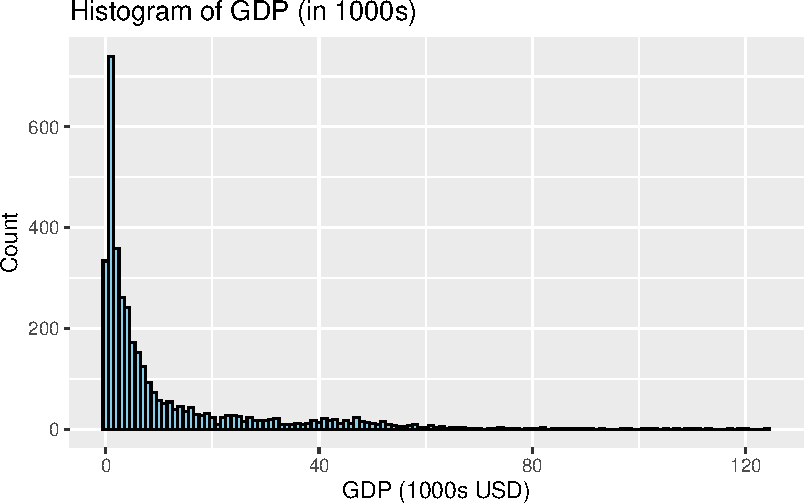
\includegraphics{EDA_files/figure-pdf/unnamed-chunk-4-1.pdf}

\begin{Shaded}
\begin{Highlighting}[]
\CommentTok{\# Population density distribution}
\FunctionTok{ggplot}\NormalTok{(data, }\FunctionTok{aes}\NormalTok{(}\AttributeTok{x =}\NormalTok{ popdens)) }\SpecialCharTok{+} 
  \FunctionTok{geom\_histogram}\NormalTok{(}\AttributeTok{binwidth =} \DecValTok{10}\NormalTok{, }\AttributeTok{fill =} \StringTok{"green"}\NormalTok{, }\AttributeTok{color =} \StringTok{"black"}\NormalTok{) }\SpecialCharTok{+}
  \FunctionTok{labs}\NormalTok{(}\AttributeTok{title =} \StringTok{"Histogram of Population Density"}\NormalTok{, }\AttributeTok{x =} \StringTok{"Population Density"}\NormalTok{, }\AttributeTok{y =} \StringTok{"Count"}\NormalTok{)}
\end{Highlighting}
\end{Shaded}

\begin{verbatim}
Warning: Removed 20 rows containing non-finite values (`stat_bin()`).
\end{verbatim}

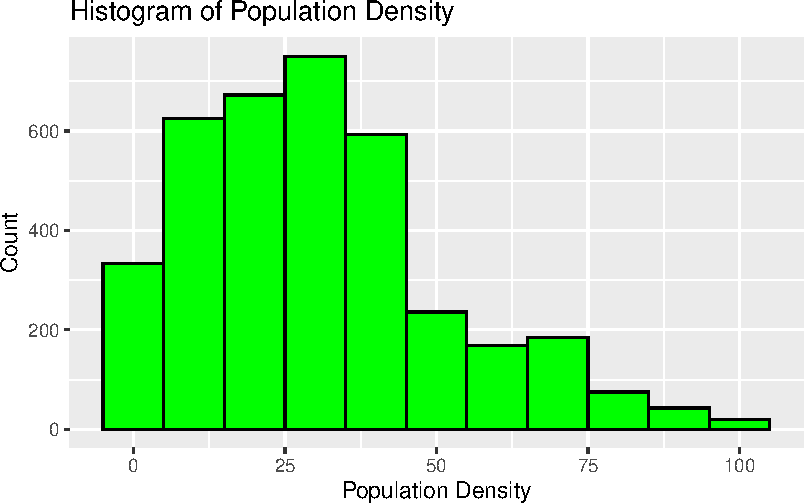
\includegraphics{EDA_files/figure-pdf/unnamed-chunk-4-2.pdf}

\textbf{Insight}: - GDP distribution is right-skewed, suggesting that
most countries have lower GDPs, while a few have significantly higher
values. - Population density also shows a right-skew, with most
countries having low-to-moderate densities and fewer countries having
high densities.

\begin{Shaded}
\begin{Highlighting}[]
\CommentTok{\# Boxplot of GDP by region}
\FunctionTok{ggplot}\NormalTok{(data, }\FunctionTok{aes}\NormalTok{(}\AttributeTok{x =}\NormalTok{ region, }\AttributeTok{y =}\NormalTok{ gdp1000, }\AttributeTok{fill =}\NormalTok{ region)) }\SpecialCharTok{+}
  \FunctionTok{geom\_boxplot}\NormalTok{() }\SpecialCharTok{+}
  \FunctionTok{labs}\NormalTok{(}\AttributeTok{title =} \StringTok{"Boxplot of GDP by Region"}\NormalTok{, }\AttributeTok{x =} \StringTok{"Region"}\NormalTok{, }\AttributeTok{y =} \StringTok{"GDP (1000s USD)"}\NormalTok{) }\SpecialCharTok{+}
  \FunctionTok{theme}\NormalTok{(}\AttributeTok{axis.text.x =} \FunctionTok{element\_text}\NormalTok{(}\AttributeTok{angle =} \DecValTok{45}\NormalTok{, }\AttributeTok{hjust =} \DecValTok{1}\NormalTok{))}
\end{Highlighting}
\end{Shaded}

\begin{verbatim}
Warning: Removed 62 rows containing non-finite values (`stat_boxplot()`).
\end{verbatim}

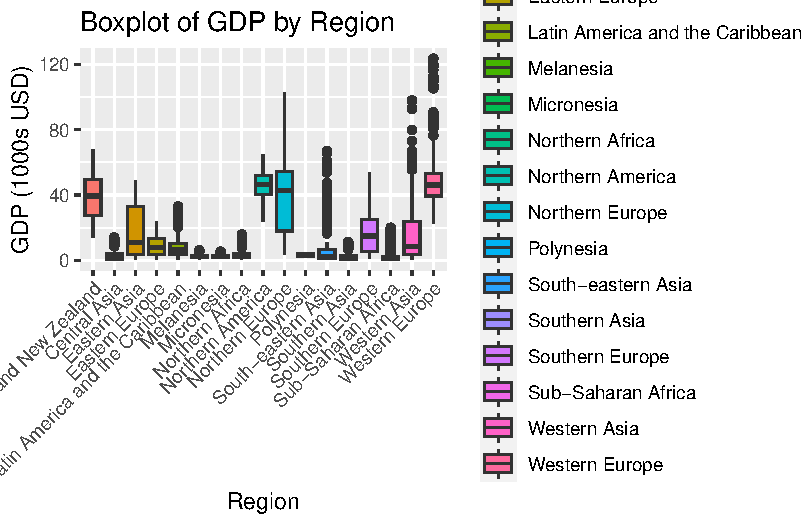
\includegraphics{EDA_files/figure-pdf/unnamed-chunk-5-1.pdf}

\textbf{Insight}: - There are notable differences in GDP across regions,
with some regions exhibiting significantly higher GDPs. The boxplot
shows high variation within regions as well, indicating economic
disparity.

\begin{Shaded}
\begin{Highlighting}[]
\CommentTok{\# Correlation matrix}
\NormalTok{corr\_matrix }\OtherTok{\textless{}{-}} \FunctionTok{cor}\NormalTok{(numeric\_vars, }\AttributeTok{use =} \StringTok{"complete.obs"}\NormalTok{)}
\FunctionTok{corrplot}\NormalTok{(corr\_matrix, }\AttributeTok{method =} \StringTok{"circle"}\NormalTok{)}
\end{Highlighting}
\end{Shaded}

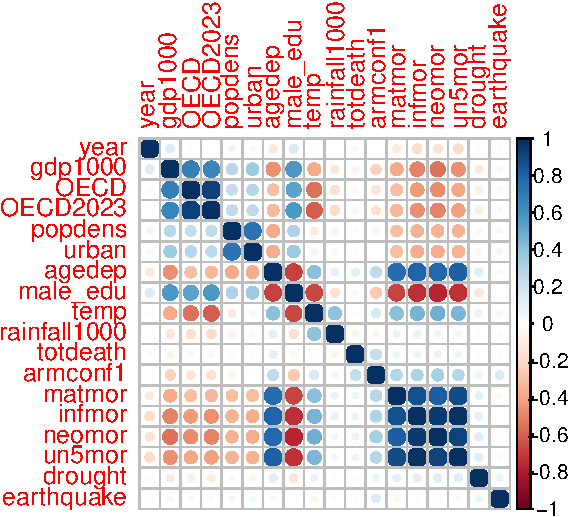
\includegraphics{EDA_files/figure-pdf/unnamed-chunk-6-1.pdf}

\textbf{Insight}: - Several numeric variables are highly correlated,
such as mortality indicators (\texttt{infmor}, \texttt{neomor},
\texttt{matmor}), which makes sense as these reflect health outcomes.

\begin{Shaded}
\begin{Highlighting}[]
\CommentTok{\# Scatterplot of GDP vs Population Density}
\FunctionTok{ggplot}\NormalTok{(data, }\FunctionTok{aes}\NormalTok{(}\AttributeTok{x =}\NormalTok{ popdens, }\AttributeTok{y =}\NormalTok{ gdp1000)) }\SpecialCharTok{+} 
  \FunctionTok{geom\_point}\NormalTok{(}\AttributeTok{alpha =} \FloatTok{0.5}\NormalTok{, }\AttributeTok{color =} \StringTok{"blue"}\NormalTok{) }\SpecialCharTok{+}
  \FunctionTok{labs}\NormalTok{(}\AttributeTok{title =} \StringTok{"Scatterplot of GDP vs Population Density"}\NormalTok{, }\AttributeTok{x =} \StringTok{"Population Density"}\NormalTok{, }\AttributeTok{y =} \StringTok{"GDP (1000s USD)"}\NormalTok{)}
\end{Highlighting}
\end{Shaded}

\begin{verbatim}
Warning: Removed 82 rows containing missing values (`geom_point()`).
\end{verbatim}

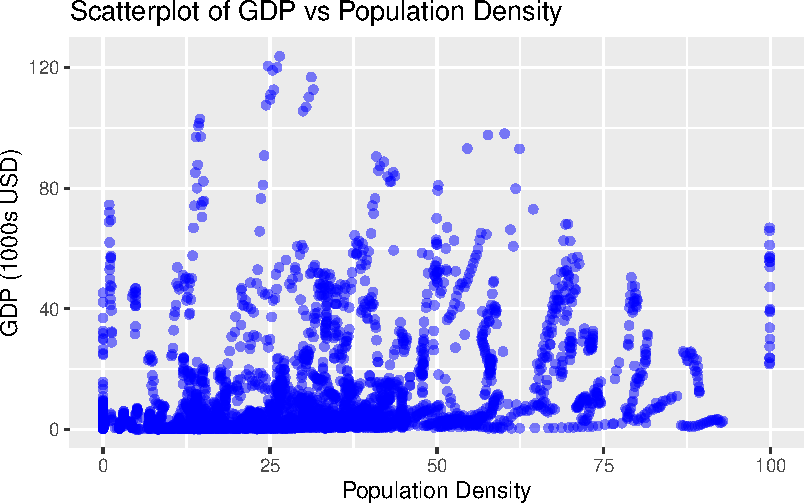
\includegraphics{EDA_files/figure-pdf/unnamed-chunk-7-1.pdf}

\textbf{Insight}: - There doesn't seem to be a strong linear
relationship between population density and GDP. This suggests that
while population density might influence GDP, other factors are more
significant.

\subsection{Regional Trends}\label{regional-trends}

\begin{Shaded}
\begin{Highlighting}[]
\CommentTok{\# Regional GDP trends over time}
\FunctionTok{ggplot}\NormalTok{(data, }\FunctionTok{aes}\NormalTok{(}\AttributeTok{x =}\NormalTok{ year, }\AttributeTok{y =}\NormalTok{ gdp1000, }\AttributeTok{color =}\NormalTok{ region)) }\SpecialCharTok{+}
  \FunctionTok{geom\_line}\NormalTok{(}\AttributeTok{stat =} \StringTok{"summary"}\NormalTok{, }\AttributeTok{fun =} \StringTok{"mean"}\NormalTok{, }\AttributeTok{size =} \FloatTok{1.2}\NormalTok{) }\SpecialCharTok{+}
  \FunctionTok{labs}\NormalTok{(}\AttributeTok{title =} \StringTok{"Average GDP over Time by Region"}\NormalTok{, }\AttributeTok{x =} \StringTok{"Year"}\NormalTok{, }\AttributeTok{y =} \StringTok{"GDP (1000s USD)"}\NormalTok{) }\SpecialCharTok{+}
  \FunctionTok{theme\_minimal}\NormalTok{()}
\end{Highlighting}
\end{Shaded}

\begin{verbatim}
Warning: Using `size` aesthetic for lines was deprecated in ggplot2 3.4.0.
i Please use `linewidth` instead.
\end{verbatim}

\begin{verbatim}
Warning: Removed 62 rows containing non-finite values (`stat_summary()`).
\end{verbatim}

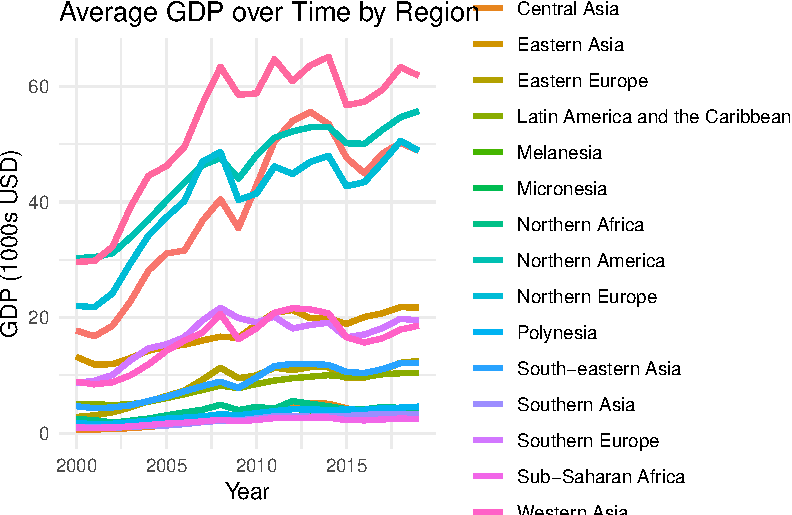
\includegraphics{EDA_files/figure-pdf/unnamed-chunk-8-1.pdf}

\textbf{Insight}: - GDP has been increasing for some regions over time,
though the rate of increase varies. Certain regions, like North America
and Europe, exhibit higher GDPs throughout.

\begin{Shaded}
\begin{Highlighting}[]
\CommentTok{\# Population density trends over time by region}
\FunctionTok{ggplot}\NormalTok{(data, }\FunctionTok{aes}\NormalTok{(}\AttributeTok{x =}\NormalTok{ year, }\AttributeTok{y =}\NormalTok{ popdens, }\AttributeTok{color =}\NormalTok{ region)) }\SpecialCharTok{+}
  \FunctionTok{geom\_line}\NormalTok{(}\AttributeTok{stat =} \StringTok{"summary"}\NormalTok{, }\AttributeTok{fun =} \StringTok{"mean"}\NormalTok{, }\AttributeTok{size =} \FloatTok{1.2}\NormalTok{) }\SpecialCharTok{+}
  \FunctionTok{labs}\NormalTok{(}\AttributeTok{title =} \StringTok{"Average Population Density over Time by Region"}\NormalTok{, }\AttributeTok{x =} \StringTok{"Year"}\NormalTok{, }\AttributeTok{y =} \StringTok{"Population Density"}\NormalTok{) }\SpecialCharTok{+}
  \FunctionTok{theme\_minimal}\NormalTok{()}
\end{Highlighting}
\end{Shaded}

\begin{verbatim}
Warning: Removed 20 rows containing non-finite values (`stat_summary()`).
\end{verbatim}

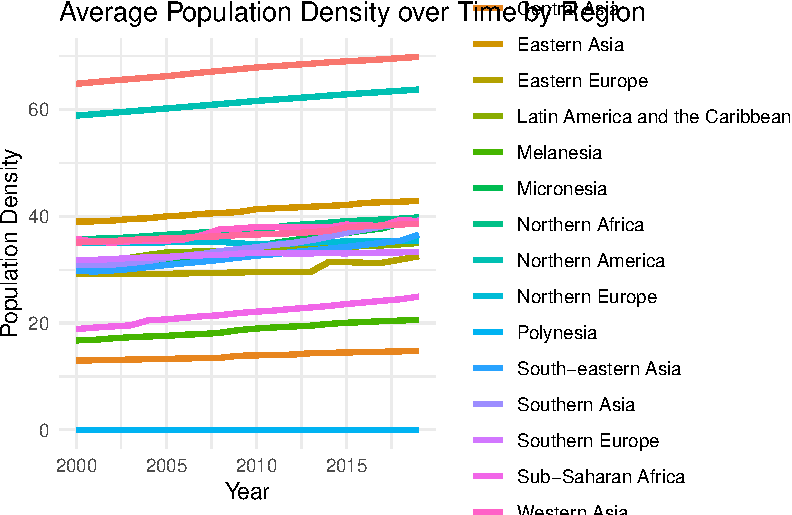
\includegraphics{EDA_files/figure-pdf/unnamed-chunk-9-1.pdf}

\textbf{Insight}: - Population density appears relatively stable over
time, with only slight variations. Some regions exhibit consistently
higher population densities.

\begin{Shaded}
\begin{Highlighting}[]
\CommentTok{\# Maternal mortality trends by region}
\FunctionTok{ggplot}\NormalTok{(data, }\FunctionTok{aes}\NormalTok{(}\AttributeTok{x =}\NormalTok{ year, }\AttributeTok{y =}\NormalTok{ matmor, }\AttributeTok{color =}\NormalTok{ region)) }\SpecialCharTok{+}
  \FunctionTok{geom\_line}\NormalTok{(}\AttributeTok{stat =} \StringTok{"summary"}\NormalTok{, }\AttributeTok{fun =} \StringTok{"mean"}\NormalTok{, }\AttributeTok{size =} \FloatTok{1.2}\NormalTok{) }\SpecialCharTok{+}
  \FunctionTok{labs}\NormalTok{(}\AttributeTok{title =} \StringTok{"Average Maternal Mortality over Time by Region"}\NormalTok{, }\AttributeTok{x =} \StringTok{"Year"}\NormalTok{, }\AttributeTok{y =} \StringTok{"Maternal Mortality (per 100,000 live births)"}\NormalTok{) }\SpecialCharTok{+}
  \FunctionTok{theme\_minimal}\NormalTok{()}
\end{Highlighting}
\end{Shaded}

\begin{verbatim}
Warning: Removed 426 rows containing non-finite values (`stat_summary()`).
\end{verbatim}

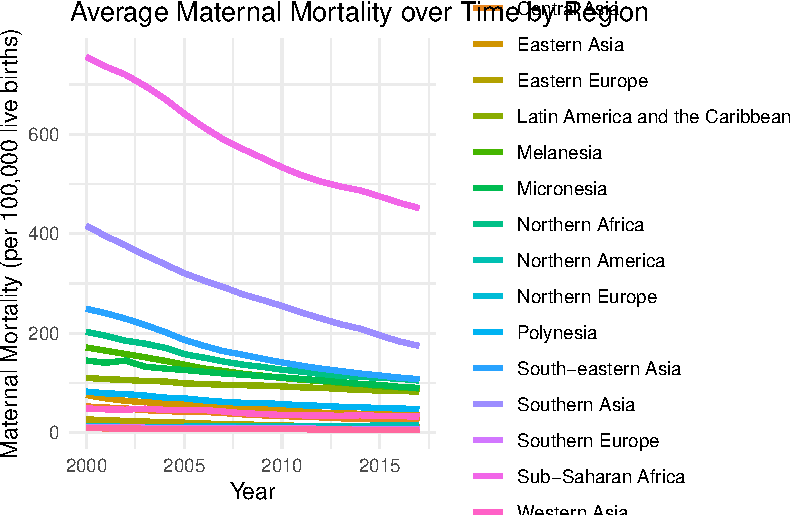
\includegraphics{EDA_files/figure-pdf/unnamed-chunk-10-1.pdf}

\textbf{Insight}: - Maternal mortality has been declining in most
regions, with significant improvements observed in certain areas like
Sub-Saharan Africa and Southern Asia.

\begin{Shaded}
\begin{Highlighting}[]
\CommentTok{\# Infant mortality trends by region}
\FunctionTok{ggplot}\NormalTok{(data, }\FunctionTok{aes}\NormalTok{(}\AttributeTok{x =}\NormalTok{ year, }\AttributeTok{y =}\NormalTok{ infmor, }\AttributeTok{color =}\NormalTok{ region)) }\SpecialCharTok{+}
  \FunctionTok{geom\_line}\NormalTok{(}\AttributeTok{stat =} \StringTok{"summary"}\NormalTok{, }\AttributeTok{fun =} \StringTok{"mean"}\NormalTok{, }\AttributeTok{size =} \FloatTok{1.2}\NormalTok{) }\SpecialCharTok{+}
  \FunctionTok{labs}\NormalTok{(}\AttributeTok{title =} \StringTok{"Average Infant Mortality over Time by Region"}\NormalTok{, }\AttributeTok{x =} \StringTok{"Year"}\NormalTok{, }\AttributeTok{y =} \StringTok{"Infant Mortality (per 1,000 live births)"}\NormalTok{) }\SpecialCharTok{+}
  \FunctionTok{theme\_minimal}\NormalTok{()}
\end{Highlighting}
\end{Shaded}

\begin{verbatim}
Warning: Removed 20 rows containing non-finite values (`stat_summary()`).
\end{verbatim}

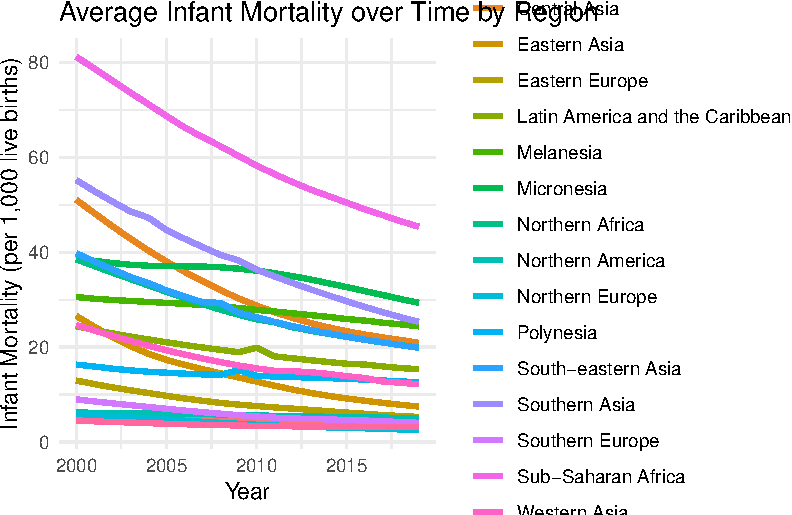
\includegraphics{EDA_files/figure-pdf/unnamed-chunk-11-1.pdf}

\textbf{Insight}: - Similar to maternal mortality, infant mortality has
been decreasing steadily across regions, although some regions still
have higher rates than others.

\begin{Shaded}
\begin{Highlighting}[]
\CommentTok{\# Neonatal mortality trends by region}
\FunctionTok{ggplot}\NormalTok{(data, }\FunctionTok{aes}\NormalTok{(}\AttributeTok{x =}\NormalTok{ year, }\AttributeTok{y =}\NormalTok{ neomor, }\AttributeTok{color =}\NormalTok{ region)) }\SpecialCharTok{+}
  \FunctionTok{geom\_line}\NormalTok{(}\AttributeTok{stat =} \StringTok{"summary"}\NormalTok{, }\AttributeTok{fun =} \StringTok{"mean"}\NormalTok{, }\AttributeTok{size =} \FloatTok{1.2}\NormalTok{) }\SpecialCharTok{+}
  \FunctionTok{labs}\NormalTok{(}\AttributeTok{title =} \StringTok{"Average Neonatal Mortality over Time by Region"}\NormalTok{, }\AttributeTok{x =} \StringTok{"Year"}\NormalTok{, }\AttributeTok{y =} \StringTok{"Neonatal Mortality (per 1,000 live births)"}\NormalTok{) }\SpecialCharTok{+}
  \FunctionTok{theme\_minimal}\NormalTok{()}
\end{Highlighting}
\end{Shaded}

\begin{verbatim}
Warning: Removed 20 rows containing non-finite values (`stat_summary()`).
\end{verbatim}

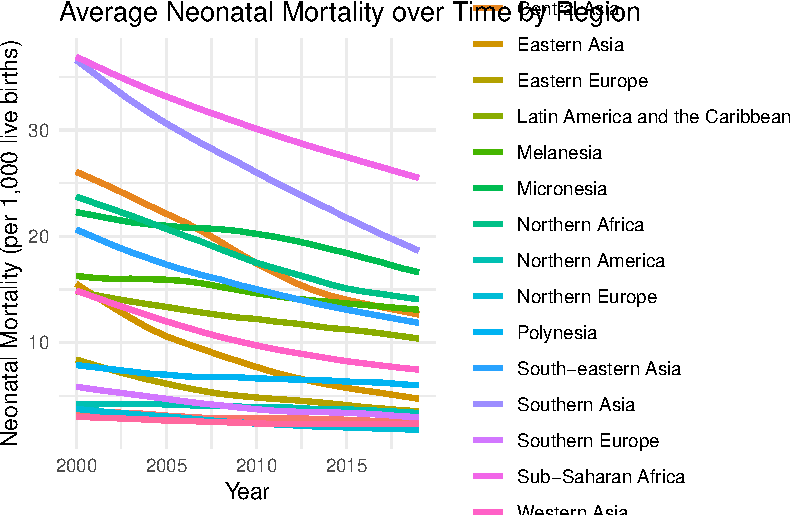
\includegraphics{EDA_files/figure-pdf/unnamed-chunk-12-1.pdf}

\textbf{Insight}: - Neonatal mortality is also declining but at a slower
pace compared to maternal and infant mortality, indicating potential
areas for further intervention in healthcare systems.

\subsection{Heatmaps}\label{heatmaps}

\begin{Shaded}
\begin{Highlighting}[]
\CommentTok{\# Heatmap for GDP by region and year}
\NormalTok{data\_gdp\_heatmap }\OtherTok{\textless{}{-}}\NormalTok{ data }\SpecialCharTok{\%\textgreater{}\%} 
  \FunctionTok{group\_by}\NormalTok{(region, year) }\SpecialCharTok{\%\textgreater{}\%}
  \FunctionTok{summarize}\NormalTok{(}\AttributeTok{mean\_gdp =} \FunctionTok{mean}\NormalTok{(gdp1000, }\AttributeTok{na.rm =} \ConstantTok{TRUE}\NormalTok{))}
\end{Highlighting}
\end{Shaded}

\begin{verbatim}
`summarise()` has grouped output by 'region'. You can override using the
`.groups` argument.
\end{verbatim}

\begin{Shaded}
\begin{Highlighting}[]
\FunctionTok{ggplot}\NormalTok{(data\_gdp\_heatmap, }\FunctionTok{aes}\NormalTok{(}\AttributeTok{x =}\NormalTok{ year, }\AttributeTok{y =}\NormalTok{ region, }\AttributeTok{fill =}\NormalTok{ mean\_gdp)) }\SpecialCharTok{+}
  \FunctionTok{geom\_tile}\NormalTok{(}\AttributeTok{color =} \StringTok{"white"}\NormalTok{) }\SpecialCharTok{+}
  \FunctionTok{scale\_fill\_gradient}\NormalTok{(}\AttributeTok{low =} \StringTok{"lightblue"}\NormalTok{, }\AttributeTok{high =} \StringTok{"darkblue"}\NormalTok{, }\AttributeTok{na.value =} \StringTok{"grey50"}\NormalTok{) }\SpecialCharTok{+}
  \FunctionTok{labs}\NormalTok{(}\AttributeTok{title =} \StringTok{"Heatmap of Average GDP by Region and Year"}\NormalTok{, }\AttributeTok{x =} \StringTok{"Year"}\NormalTok{, }\AttributeTok{y =} \StringTok{"Region"}\NormalTok{, }\AttributeTok{fill =} \StringTok{"Mean GDP (1000s USD)"}\NormalTok{) }\SpecialCharTok{+}
  \FunctionTok{theme\_minimal}\NormalTok{()}
\end{Highlighting}
\end{Shaded}

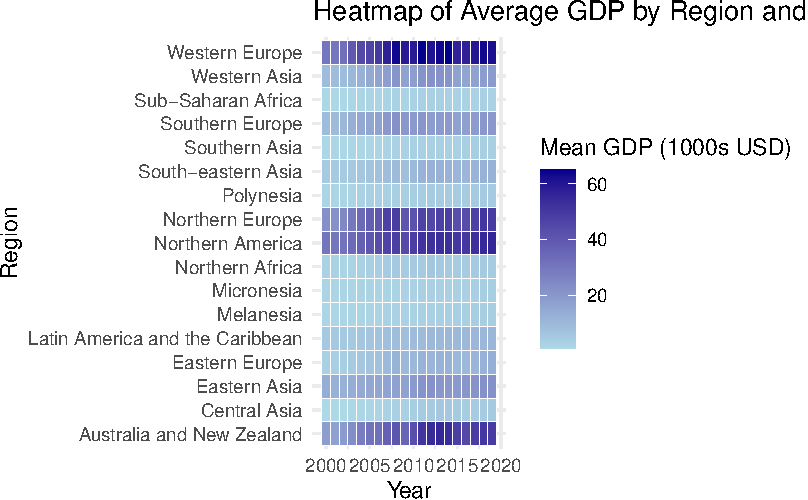
\includegraphics{EDA_files/figure-pdf/unnamed-chunk-13-1.pdf}

\textbf{Insight}: - The heatmap shows consistent GDP growth in regions
like North America and Europe, while other regions like Africa and
Southern Asia lag behind.

\begin{Shaded}
\begin{Highlighting}[]
\CommentTok{\# Heatmap for Population Density by region and year}
\NormalTok{data\_popdens\_heatmap }\OtherTok{\textless{}{-}}\NormalTok{ data }\SpecialCharTok{\%\textgreater{}\%} 
  \FunctionTok{group\_by}\NormalTok{(region, year) }\SpecialCharTok{\%\textgreater{}\%}
  \FunctionTok{summarize}\NormalTok{(}\AttributeTok{mean\_popdens =} \FunctionTok{mean}\NormalTok{(popdens, }\AttributeTok{na.rm =} \ConstantTok{TRUE}\NormalTok{))}
\end{Highlighting}
\end{Shaded}

\begin{verbatim}
`summarise()` has grouped output by 'region'. You can override using the
`.groups` argument.
\end{verbatim}

\begin{Shaded}
\begin{Highlighting}[]
\FunctionTok{ggplot}\NormalTok{(data\_popdens\_heatmap, }\FunctionTok{aes}\NormalTok{(}\AttributeTok{x =}\NormalTok{ year, }\AttributeTok{y =}\NormalTok{ region, }\AttributeTok{fill =}\NormalTok{ mean\_popdens)) }\SpecialCharTok{+}
  \FunctionTok{geom\_tile}\NormalTok{(}\AttributeTok{color =} \StringTok{"white"}\NormalTok{) }\SpecialCharTok{+}
  \FunctionTok{scale\_fill\_gradient}\NormalTok{(}\AttributeTok{low =} \StringTok{"lightgreen"}\NormalTok{, }\AttributeTok{high =} \StringTok{"darkgreen"}\NormalTok{, }\AttributeTok{na.value =} \StringTok{"grey50"}\NormalTok{) }\SpecialCharTok{+}
  \FunctionTok{labs}\NormalTok{(}\AttributeTok{title =} \StringTok{"Heatmap of Population Density by Region and Year"}\NormalTok{, }\AttributeTok{x =} \StringTok{"Year"}\NormalTok{, }\AttributeTok{y =} \StringTok{"Region"}\NormalTok{, }\AttributeTok{fill =} \StringTok{"Mean Pop. Density"}\NormalTok{) }\SpecialCharTok{+}
  \FunctionTok{theme\_minimal}\NormalTok{()}
\end{Highlighting}
\end{Shaded}

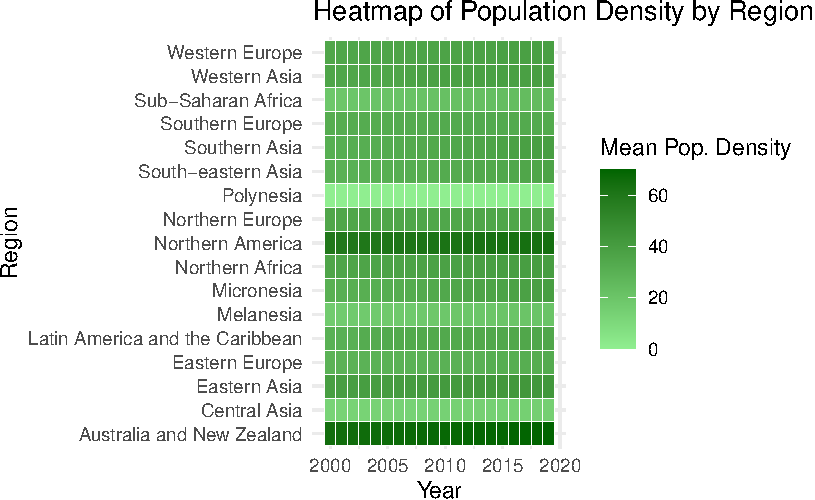
\includegraphics{EDA_files/figure-pdf/unnamed-chunk-14-1.pdf}

\textbf{Insight}: - The population density heatmap highlights regions
with higher densities, such as Southern Asia and Sub-Saharan Africa,
while other regions have more sparse populations.

\begin{Shaded}
\begin{Highlighting}[]
\CommentTok{\# Comparing multiple mortality indicators by region}
\NormalTok{mortality\_data }\OtherTok{\textless{}{-}}\NormalTok{ data }\SpecialCharTok{\%\textgreater{}\%} 
  \FunctionTok{select}\NormalTok{(region, year, matmor, infmor, neomor, un5mor) }\SpecialCharTok{\%\textgreater{}\%}
  \FunctionTok{gather}\NormalTok{(}\AttributeTok{key =} \StringTok{"mortality\_type"}\NormalTok{, }\AttributeTok{value =} \StringTok{"mortality\_rate"}\NormalTok{, matmor, infmor, neomor, un5mor)}

\FunctionTok{ggplot}\NormalTok{(mortality\_data, }\FunctionTok{aes}\NormalTok{(}\AttributeTok{x =}\NormalTok{ year, }\AttributeTok{y =}\NormalTok{ mortality\_rate, }\AttributeTok{color =}\NormalTok{ region)) }\SpecialCharTok{+}
  \FunctionTok{geom\_line}\NormalTok{(}\AttributeTok{stat =} \StringTok{"summary"}\NormalTok{, }\AttributeTok{fun =} \StringTok{"mean"}\NormalTok{, }\AttributeTok{size =} \FloatTok{1.2}\NormalTok{) }\SpecialCharTok{+}
  \FunctionTok{facet\_wrap}\NormalTok{(}\SpecialCharTok{\textasciitilde{}}\NormalTok{mortality\_type, }\AttributeTok{scales =} \StringTok{"free\_y"}\NormalTok{) }\SpecialCharTok{+}
  \FunctionTok{labs}\NormalTok{(}\AttributeTok{title =} \StringTok{"Mortality Trends by Region (Various Indicators)"}\NormalTok{, }\AttributeTok{x =} \StringTok{"Year"}\NormalTok{, }\AttributeTok{y =} \StringTok{"Mortality Rate"}\NormalTok{) }\SpecialCharTok{+}
  \FunctionTok{theme\_minimal}\NormalTok{()}
\end{Highlighting}
\end{Shaded}

\begin{verbatim}
Warning: Removed 486 rows containing non-finite values (`stat_summary()`).
\end{verbatim}

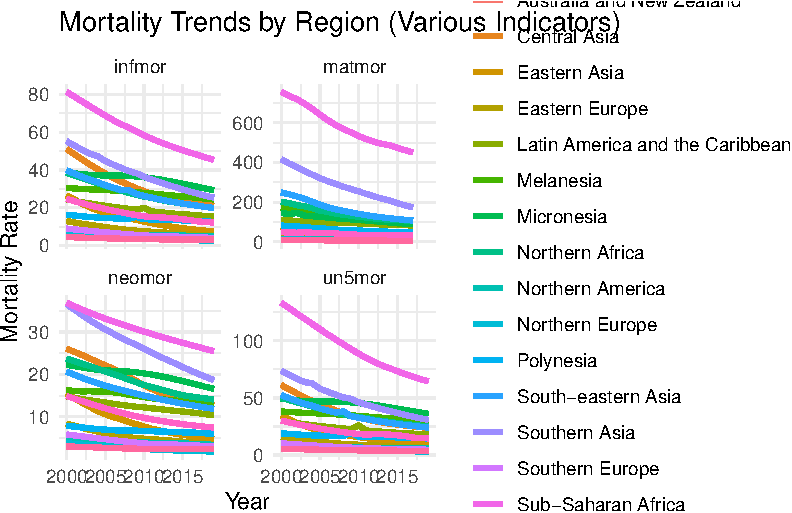
\includegraphics{EDA_files/figure-pdf/unnamed-chunk-15-1.pdf}

\textbf{Insight}: - This visualization clearly shows the downward trend
in mortality




\end{document}
